In computational linear algebra, we would spend a lot of time in matrix equations or expressions like $Ax = b$. However, for large matrices  $A$, it is always difficult and inefficient to find the value of $x$, if we try finding the inverse of $A$ directly. So what we want to do is to "transform" our $A$ into smaller building blocks with specific properties, and use the properties of them to make the equation easier to solve. 

\medskip
\noindent The transformations, should preserve the correctness in matrix calculations (be sufficiently free from truncation errors, as said in the \href{https://comp-lin-alg.github.io/L2_QR_factorisation.html#what-is-the-qr-factorisation}{\textbf{Introduction}} of Chapter 2), and be efficient enough to perform. Here, let us talk about the very first transformation, the \textbf{QR Factorisation}. 
\medskip

\noindent You might have seen this in your year 2 \href{https://github.com/Imperial-MATH50003/MATH50003NumericalAnalysis}{Numerical Analysis} Course, and make some progress in implementation using Julia or Python. We would do some recap and dig further in algorithm stability, and/or time complexities with different ways of implementations.

\section{QR Factorisation Concept}%
What does \textbf{QR Factorisation} do is to simply decompose an arbitrary matrix $A$, to a unitary matrix $Q$ and an upper triangular matrix $R$. 
i.e. to  write
\[
  A = QR \text{ where } A \in \mathbb{C}^{m\times n}, Q  \text{ unitary } \in \mathbb{C}^{m \times m}, R  \text{ upper triangular } \in \mathbb{C}^{m \times n}
.\]
And without loss of generality we consider $m > n$, and have:
\[
\underset{\begin{array}{c}\\ A \end{array}}%
{
\begin{pmatrix}
  a_{11} & a_{12} & \ldots & a_{1n} \\
  a_{21} & a_{22} & \ldots & a_{2n} \\
  \vdots & \vdots & \ddots & \vdots \\
  a_{m1} & a_{m2} & \ldots & a_{mn}
\end{pmatrix}
}
=
\underset{\begin{array}{c}\\ Q \end{array}}%
{
\begin{pmatrix}
  q_{11} & q_{12} & \ldots & q_{1n} & \ldots & q_{1m} \\
  q_{21} & q_{22} & \ldots & q_{2n} & \ldots & q_{2m}\\
  \vdots & \vdots & \ddots & \vdots & \ddots & \vdots\\
  q_{m1} & q_{m2} & \ldots & q_{mn} & \ldots & q_{mm}
\end{pmatrix}
}
\begin{spmatrix}{R}
  r_{11} & r_{12} & \ldots & r_{1n} \\
  0 & r_{22} & \ldots & r_{2n} \\
  0 & 0 & \ldots & r_{3n} \\
  \vdots & \vdots & \ddots & \vdots \\
  0 & 0 & \ldots & r_{nn} \\
  \vdots & \vdots & \ddots & \vdots \\
  0 & 0 & \ldots & 0
\end{spmatrix}
\] 
And we called this as the \textbf{complete QR factorisation}. 

\medskip

\noindent Note that, the term $q_{ik}r_{kj}$ would always give out 0 as result when $k > n$ and make no contribution to the value of  $a_{ij}$. Therefore, we could only consider the first $n$ columns of $Q$, $\hat{Q}$ and the first $n$ rows of  $R$,  $\hat{R}$ as result of factorisation instead (i.e. Determine $A = \hat{Q}\hat{R}$ as a reduced alternative).

\subsection*{Exercise 2.3: Find an orthonormal basis of the orthogonal complement of a subspace}
\addcontentsline{toc}{subsection}{Exercise 2.3: Find an orthonormal basis of the orthogonal complement of a subspace}
\subsubsection*{Problem Description}%
\label{ssub:problem_description}

Given a set of vectors $ \{v_1, v_2, \ldots, v_n\}$ spans subspace $U \subset \mathbb{C}^{m}$, we need to find an orthonormal basis of its orthogonal complement $U^{\bot}$, defined as:
\[
U^{\bot} = \{x \in \mathbb{C}^{m}: \forall u \in U, x^{*}u = 0\} 
.\] 
Implement this as a function \href{https://comp-lin-alg.github.io/cla_utils.html#cla_utils.exercises2.orthog_space}{\texttt{exercises2.orthog\_space()}}. \medskip

\noindent  
(hint: You should make use of the built in QR factorisation routine

\noindent \texttt{numpy.linalg.qr()}.)

\subsubsection*{What to do}%
\label{ssub:what_to_do}

\begin{enumerate}
  \item Think about what does QR factorisation actually do: what are the properties of $Q$ and $R$  (and similarly $\hat{Q}$ and $\hat{R}$ in the reduced version)?
  \item You might notice $Q$ (and $\hat{Q}$) is unitary, so try to think about the relationship between column vectors in matrix by expanding $Q^*Q = I$.
  \item And the basis of $U$ could be easily seen by the columns of $\hat{Q}$. So if we find the vectors orthogonal to all column vectors in $\hat{Q}$, we should find the basis of the orthogonal complement of $U$.
  \item Go back to step 2 and see if you can find vectors orthogonal to columns of \(\hat{Q}\) from some certain matrices. Make the implementation in Python.
\end{enumerate}
\noindent \textbf{Remember to check your implementation pass the provided test cases.}
\subsubsection*{Spoil Alert\ldots There is a way you could figure out the problem}%
\label{ssub:analysis}
Here we have some explanation to this implementation:
\begin{itemize}
\item Given that we know $Q$ is unitary, we would see all column vectors are orthogonal to each other by expanding
  \[
    [Q^*Q]_{ij} = q_i^*q_j = I_{ij} = \left\{
      \begin{array}{l}
      0 \text{ when $i \neq j$} \\
      1 \text{ when $i = j$}
      \end{array}
    \right.
  .\] 
  \item And since we need to find the vectors that orthogonal to all column vectors in $\hat{Q}$, which is the first $n$ columns of $Q$. We could actually see the remaining $m - n$ columns in  $Q$ are actually orthogonal to all column vectors in $\hat{Q}$, by the mutual orthogonality we observed in column space of $Q$. 
  \item Therefore, what we need to do is just to find the value of Q. And we need to get the \textbf{last} $m - n$ \textbf{columns} from $Q$, which should should be the basis of the orthogonal complementary $U^{\bot}$.
\end{itemize}

\newpage
\section{QR factorisation by classical Gram-Schmidt}%
We have already seen the concept of QR factorisation, and one of the application through the previous exercise. Then we are going to explore what exactly happens in this factorisation, via algorithms. The first implementation we would discuss would be the \textbf{classical Gram-Schmidt algorithm}. 

\medskip
\noindent But before we just show the explicit implementation, we could look backwards to see how vectors $ \{a_i\} $ factctorised to orthonormal vectors $ \{q_i\} $. Just expand $A = QR$ by arithmetic:

 \[
   A = QR \implies \begin{pmatrix} a_1 & a_2 & \ldots & a_n \end{pmatrix} = 
   \begin{pmatrix} 
     q_1 & q_2 & \ldots & q_n 
  \end{pmatrix} 
   \begin{pmatrix} 
     r_{11} & r_{12} & \ldots & r_{1n} \\ 
     0 & r_{22} & \ldots & r_{2n} \\
     \vdots & \vdots & \ddots & \vdots \\
     0 & 0 & \ldots & r_{nn}
   \end{pmatrix}  
.\] 
So we could see the value of any column vector $a_j$ via column-space interpretation and get:
\[
  a_j = 
   \begin{pmatrix} 
     q_1 & q_2 & \ldots & q_j & \ldots & q_n 
  \end{pmatrix} 
  \begin{pmatrix} r_{1j}\\ r_{2j} \\ \vdots\\ r_{jj} \\ 0 \\ \vdots \\ 0 \end{pmatrix}
\] 
\[
  = r_{1j} q_1 + r_{2j}q_2 + r_{3j}q_3 + \ldots + r_{jj}q_j + 0 \cdot q_{j + 1} + \ldots + 0
  = \sum_{i=1}^{j} r_{ij}q_i
.\] 
Starting with $a_1$, we could see that:
 \[
a_1 = r_{11} q_1
.\] 
and in this expression we could observe $q_1$ is the unit vector parallel to $a_1$, so $r_{11}$ and $q_1$ should have the value
\[
r_{11} = \|a_1\| \text{ and } q_1 = \frac{a_1}{\|a_1\|} = \frac{a_1}{r_{11}}
.\]
Then consider $a_2$ from the summation expression above:
 \[
a_2 = r_{12}q_1 + r_{22}q_2
.\]
But we don't know how to get the value of $r_{12}$ yet. Recall the idea we used in the implementation of $\texttt{orthog\_cpts()}$, we have now have a one-element only orthonormal set $ \{q_1\} $, we need to compute $a_2 = r' + u_1q_1 = r_{22}q_2 + r_{12}q_1$. So simply we see
\[
  r_{12} = u_1 = q_1^* a_2
\]
and to get the value of $q_2$ and $r_{22}$, we remove the component of $q_1$ from $a_2$ and we could get:
\[
    v_2 = a_2 - r_{12}q_1 = r_{22}q_2 \implies 
    \left\{
      \begin{array}{l}
      r_{22} = \|v_2\| \\
      q_2 = \frac{v_2}{\|v_2\|} = \frac{v_2}{r_{22}}
      \end{array}
    \right.
.\]
Then we could add $q_2$ to the orthonormal set and use $ \{q_1, q_2\} $ to compute corresponding $q_3$ and scale factor $r_{i3}$s. And as we repeat these steps iteratively, we could compute the value of $q_4, q_5, \ldots$ until $q_n$. \medskip

\noindent And more generally, given matrix \(A \in \mathbb{C}^{m \times n}\), we could compute the entries of \(Q \in \mathbb{C}^{m \times  n}, R \in \mathbb{C}^{n \times  n}\) with the following formula:
\[
  q_i = \frac{v_{i}}{\|v_{i}\|}
.\]
\[
  r_{ij} = \left\{
    \begin{array}{ll}
    q_{i}^{*}a_{j} & i < j\\
    \|v_{j}\| & i = j\\
    0 & \text{otherwise}
    \end{array}
  \right.
.\]
where
\[
  v_{i} = \left\{
      \begin{array}{ll}
      a_{i} & i = 1\\
      a_{i} - \sum_{k=1}^{i - 1} r_{ki}q_{k} = a_{i} - \sum_{k=1}^{i - 1} (q_{k}q_{k}^{*})a_{i} & \text{otherwise}
      \end{array}
  \right.
.\]
And then the explicit algorithm of QR factorisation via classical Gram-Schmidt should be very straightforward. You can find it \href{https://comp-lin-alg.github.io/L2_QR_factorisation.html#qr-factorisation-by-classical-gram-schmidt-algorithm}{here} from master notes and step in to the very first implementation exercise of QR.
\newpage

\noindent To be more specific, \autoref{cgs} would demonstrate the flow of the classical Gram-Schmidt Algorithm, if we just focus on turning \(A\) to \(Q\): 
\begin{figure}[htp]
  \centering
  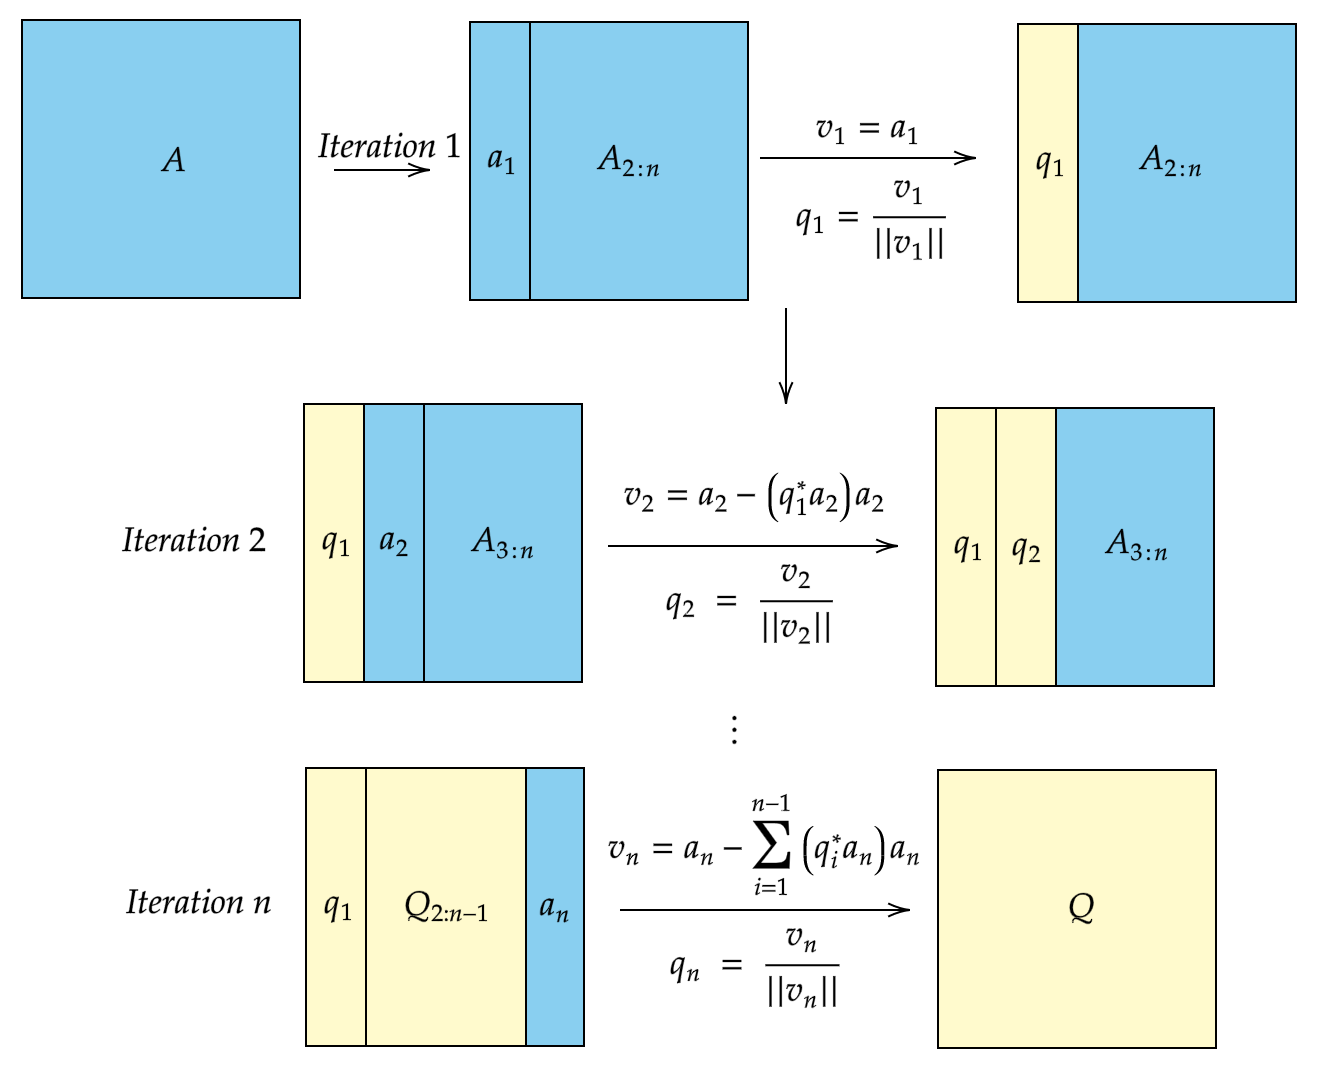
\includegraphics[width=\textwidth]{imgs/cgs.png}
  \caption{Classical Gram-Schmidt Algorithm Demonstration}
  \label{cgs}
\end{figure}
\subsection*{Exercise 2.4: Implement the Gram-Schmidt Algorithm}
\addcontentsline{toc}{subsection}{Exercise 2.4: Implement the classical Gram-Schmidt Algorithm}
\subsubsection*{Problem Description}%
Here you need to implement the classical Gram-Schmidt algorithm from the derivation above in your function \href{https://comp-lin-alg.github.io/cla_utils.html#cla_utils.exercises2.GS_classical}{\texttt{exercises2.GS\_classical()}}. Note that instead returning matrices \(Q\) and \(R\) from the function, you need to change original matrix \(A\) to \(Q\) 'in-place', and return \(R\) only.
\subsubsection*{What to do}
There is not too much to say about this exercise. Try using 'vectorized' operations in your implementation, e.g. matrix multiplication rather than additional loops. \medskip

\noindent \textbf{Remember to check your implementation pass the provided test cases.}